\section{Linux namespaces}
\label{sec:intro:containerization:linux_namespaces}
A Linux namespace encloses a global system resource in an abstraction that makes the processes within the namespace appear to have their own isolated instance of the global resource. Changes to the global resource are visible to other processes that are members of the namespace, but invisible to other processes. Namespaces are the basic building block of containers under Linux. There are the following namespaces available under Linux:
\begin{itemize}
\item Cgroup
\item Interprocess communication (IPC)
\item Network
\item Mount
\item PID
\item User
\item UTS
\end{itemize}

It doesn't make any sense to describe every namespace in detail. In the following only essential namespaces are explained.

\subsection{Mount}
\label{sec:intro:containerization:linux_namespaces:mount_namespaces}
Mount namespaces provide an isolation of the list of mount points seen by the processes in each namespace instance. Thus, the processes in each of the mount namespace instances see different single views of directory hierarchies. This view can range from physical or network drives, mount paths, or advanced features such as union file systems which are discussed in \ref{sec:intro:docker_image:unionfs}.

\subsection{IPC}
\label{sec:intro:containerization:linux_namespaces:ipc_namespaces}
IPC namespaces isolate certain IPC resources like System V IPC objects and POSIX message queues which both are data structures which allows via e.g. shared memory to transfer information between processes.

\subsection{PID}
\label{sec:intro:containerization:linux_namespaces:pid_namespaces}
Traditional the Linux kernel has always maintained a single process tree. The tree contains a reference to each process currently running in a parent-child hierarchy. 
Each time a Linux system starts, it starts with only process PID1. This process is the root of the process tree and initiates the rest of the system by starting different handlers and services. All other processes start below this process in the tree. The basic idea behind PID namespaces are to create and append a new root tree to the already existing tree with its own PID1. This makes the child process to a root process itself.
With PID namespace isolation, the processes in the lower-level namespace have no possibility of detecting the existence of the higher-level process. This ensures that processes that belong to a process tree do not inspect or kill processes in other process trees of siblings or higher-level processes. However, processes in the higher-level namespace have a full view in the lower-level namespace of processes, as if they were another process in the higher-level namespace.

\subsection{Network}
\label{sec:intro:containerization:linux_namespaces:network_namespaces}
Due to the global instance of that network interface on a single host it is possible across the whole operating system to create or edit routing + arp table entries with correct granted permissions. With network namespaces, it is possible to have totally different instances of network interfaces and routing + arp tables that operate independent of each other. This prevents communication between network namespaces.
 
Network namespaces are complex, but important to know in order to remove partially the isolation and establish communication between containers and hosts, and between containers themselves. 
The following list shows the standardized CNI (Container Network Interface) workflow, how network namespaces are created and how a desired communication between these namespaces can be established.

\begin{enumerate}
\item Create network namespace
\item Create bridge Network/Interface
\item Create veth pairs
\item Attach veth to namespace and bridge
\item Assign IP addresses
\item Bring interfaces up
\end{enumerate}

For a better understanding, an example with 2 network namespaces is shown in Figure \ref{sec:intro:containerization:linux_namespaces:netowork_ns} below. Each color represents a network namespace with its associated virtual network interface pairs(veth-x and veth-x.bridge). For simplicity IP addresses are not shown in this image. C1 in this picture is just a prefix for the underlying host which is arbitrary in this case. Basically, communication between any networks from a view of a network namespace is not possible as already mentioned. Network communication across namespaces is allowed after the CNI procedure. Finally the two interface endpoints (purple and orange) have a valid IP address which leads to a working network communication.

\begin{figure}[htbp]
 \centering
 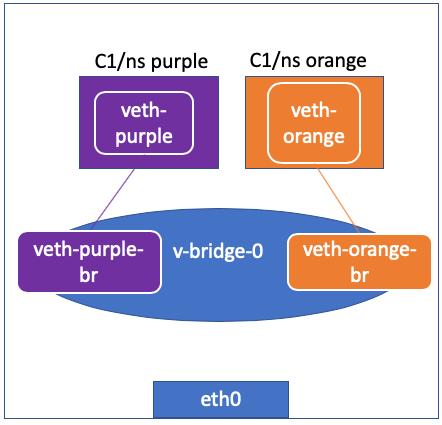
\includegraphics[width=0.4\textwidth]{gfx/examples/network_ns}
 \caption{Example of basic network within a container cluster}
\label{sec:intro:containerization:linux_namespaces:netowork_ns}
\end{figure}

This is just the beginning of network communication through namespaces and CNI. But just inter communication between different namespaces on a single host isn't sufficient. Several steps are required to communicate with another host externally and over the Internet.

Figure \ref{sec:intro:containerization:linux_namespaces:netowork_ns_ou} shows a more comprehensive setup. 
There is shown that the local host is also the gateway because it has one network connection through the interface eth0 and it has access to the bridge network created on the host. If the blue namespace network wants to access the endpoint with the IP address 192.168.1.3, there is a routing table entry in the blue network namespace like the following necessary 

\begin{lstlisting}
	ip netns exec blue ip route add 192.168.1.0/24 via 192.168.15.5
\end{lstlisting}

This allows only one direction, from the namespace to the outside endpoint. To enable access from outside to this network namespace it is necessary to create a NAT rule via iptables.

\begin{lstlisting}
	iptables -t nat -A POSTROUTING -s 192.168.15.0/24 -j MASQUERADE	
\end{lstlisting}

In order to provide access to the internet from a namespace its just necessary to add a default route

\begin{lstlisting}
	ip netns exec blue ip rout add default via 192.168.15.5
\end{lstlisting}

\begin{figure}[htbp]
 \centering
 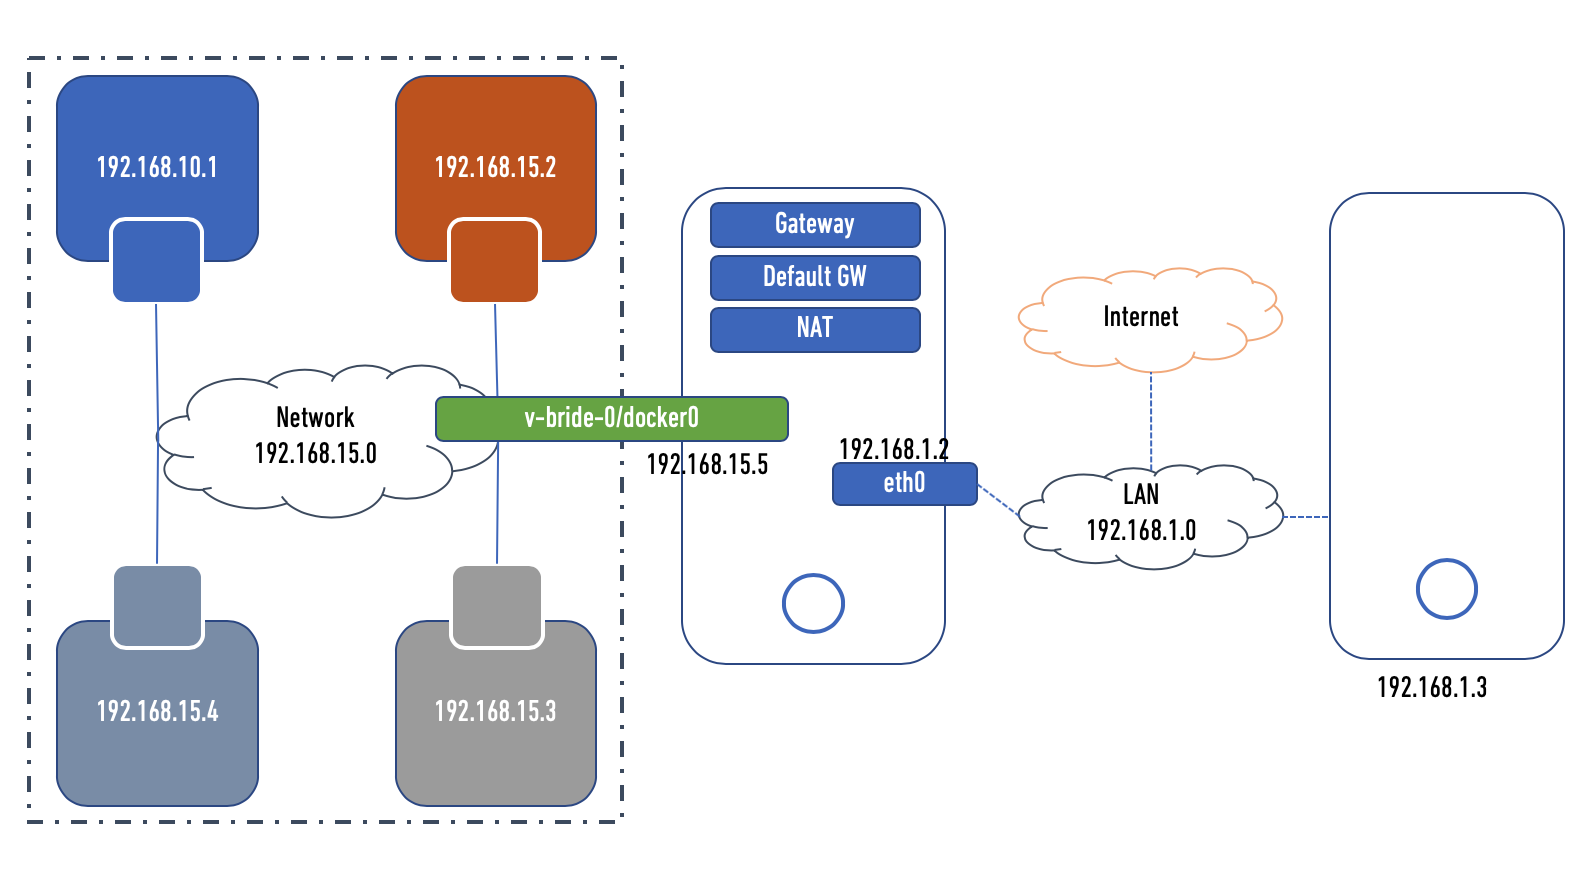
\includegraphics[width=0.7\textwidth]{gfx/examples/network_ns_out}
 \caption{Example of comprehensive networking within and outside of container}
\label{sec:intro:containerization:linux_namespaces:netowork_ns_out}
\end{figure}

This example of network namespaces, which are associated to different processes, shows the power and flexibility of network namespaces.
Normally these manual steps are done through CLI via a daemon like Docker. This in turn can be managed by an orchestrator like Kubernetes or Mesos.

At next there is just one Linux namespace left, the user namespace.

\subsection{User}
\label{sec:intro:containerization:linux_namespaces:user_namespaces}
User Namespaces insulates user and group IDs so they appear different both inside and outside the user namespace.
User namespaces give processes the ability to believe that they are working as root when they are inside the namespace. In addition it appears as if another process is being executed by a user with low permissions.
User namespaces can also operate on capabilities and privileges. 
What are capabilities? In contrast to privileged processes that bypass all kernel permission checks, unprivileged processes have to pass full permission checking based on the process’s credentials such as effective UID, GID and supplementary group list. Linux today has privileged process rights divided into different units called capabilities. These distinct units/privileges can be independently assigned and enabled for unprivileged processes.

The next section describes in short another Linux kernel feature, called cgroups, which provide another level of security in order to provide a smooth working container environment.

\section{Cgroups}
\label{sec:intro:containerization:cgroups}
Control groups (Cgroups) are a way of enforcing hardware resource limitations and access controls on a process or set of processes. The cgroup scheme provide a hierarchical, inheritable, and optionally nested resource control mechanism.
In the world of containers, cgroups obviously manifest themselves as instruments to prevent runaway containers and denial of service attacks.
The following lists contain the resources are controlled via cgroups

\begin{itemize}
\item CPU usage
\item Memory usage
\item Disk usages
\item Device whitelist
\item Network traffic based on tags(class id value) and iptables for filtering
\item Application freeze and unfreeze by sending special signals
\item PID limitation to limit a specific amount of processes 
\end{itemize}

After this section, awareness is gained that containers can work isolated just via Linux native functions.
The next important section gives an architectural introduction to the root of every container - a container image.
